\chapter*{Perulangan "Apa Kabar" sejumlah 2 digit NPM }

\par
Kita bisa melakukan hal tersebut dengan inputan dari user yang membuat variabel, pengulangannya oleh batas range yang sudah diatur. Caranya sebagai berikut :


\begin{enumerate}
   

\item buka spyder dan ketikan kode seperti berikut
	\begin{figure} [h]
	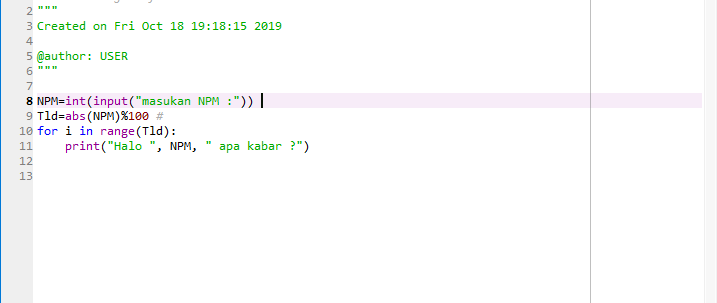
\includegraphics[width=10cm]{pakabs/pakabs.png}
	\centering
	\end{figure}
	
	
	
 \item maka akan tercetak 
 \begin{figure} [h]
	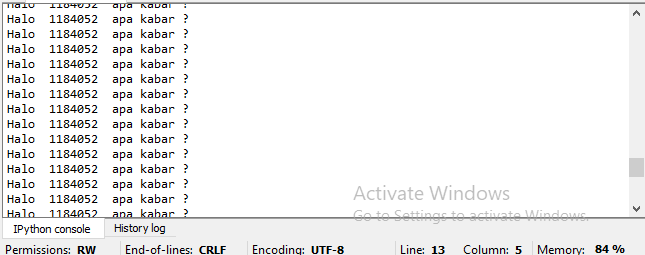
\includegraphics[width=9cm]{pakabs/pakabs2.png}
	\centering
	\end{figure}
 
	
	\end{enumerate}